\documentclass[12pt,a4paper]{article}
\usepackage[top=1.5cm, bottom=1.5cm, left=2.0cm, right=1.5cm] {geometry}
\usepackage{amsmath,amssymb,txfonts}
\usepackage{tkz-euclide}
\usepackage{setspace}
\usepackage{lastpage}

\usepackage{tikz,tkz-tab}
%\usepackage[solcolor]{ex_test}
%\usepackage[dethi]{ex_test} % Chỉ hiển thị đề thi
\usepackage[loigiai]{ex_test} % Hiển thị lời giải
%\usepackage[color]{ex_test} % Khoanh các đáp án
\everymath{\displaystyle}

\def\colorEX{\color{purple}}
%\def\colorEX{}%Không tô màu đáp án đúng trong tùy chọn loigiai
\renewtheorem{ex}{\color{violet}Câu}
\renewcommand{\FalseEX}{\stepcounter{dapan}{{\bf \textcolor{blue}{\Alph{dapan}.}}}}
\renewcommand{\TrueEX}{\stepcounter{dapan}{{\bf \textcolor{blue}{\Alph{dapan}.}}}}

%---------- Khai báo viết tắt, in đáp án
\newcommand{\hoac}[1]{ %hệ hoặc
    \left[\begin{aligned}#1\end{aligned}\right.}
\newcommand{\heva}[1]{ %hệ và
    \left\{\begin{aligned}#1\end{aligned}\right.}

%Tiêu đề
\newcommand{\tenso}{iMath}
\newcommand{\tentruong}{Phần mềm Tạo đề ngẫu nhiên}
\newcommand{\tenkythi}{ĐỀ ÔN TẬP}
\newcommand{\tenmonthi}{Môn thi: Toán}
\newcommand{\thoigian}{}
\newcommand{\tieude}[1]{
   \begin{tabular}{cm{3cm}cm{3cm}cm{3cm}}
    {\bf \tenso} & & {\bf \tenkythi} \\
    {\bf \tentruong} & & {\bf \tenmonthi}\\
    && {\bf Thời gian: \bf \thoigian \, phút}\\
    && { \fbox{\bf Mã đề: #1}}
   \end{tabular}\\\\
    
   {Họ tên HS: \dotfill Số báo danh \dotfill}\\
}
\newcommand{\chantrang}[2]{\rfoot{Trang \thepage $-$ Mã đề #2}}
\pagestyle{fancy}
\fancyhf{}
\renewcommand{\headrulewidth}{0pt} 
\renewcommand{\footrulewidth}{0pt}

\begin{document}
%Thiết lập giãn dọng 1.5cm 
%\setlength{\lineskip}{1.5em}
%Nội dung trắc nghiệm bắt đầu ở đây


\tieude{001}
\chantrang{\pageref{LastPage}}{001}
\setcounter{page}{1}
\begin{ex}
	Cho tứ diện ${BCEF}$. Gọi ${P,J,N}$ lần lượt là trung điểm của ${BC,CE,BF}$. Khẳng định nào sau đây là khẳng định đúng? 
	\begin{center}
		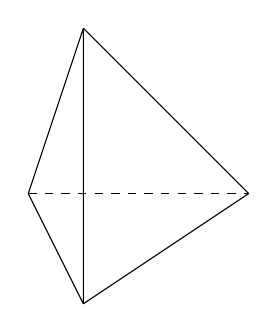
\begin{tikzpicture}[scale=0.7]
			\coordinate (C) at (0,0);
			\coordinate (E) at (1,-2);
			\coordinate (F) at (4,0);
			\coordinate (B) at (1,3);
			\draw [dashed] (C)--(F); 
			\draw (C)--(E) (E)--(F) (B)--(C) (B)--(E) (B)--(F);
		\end{tikzpicture}
		
	\end{center}
	\choice
	{ $EF//(BPJ)$ }
	{ \True $PN//(JEF)$ }
	{ $EP//(BJF)$ }
	{ $FJ//(BCE)$ }
	\loigiai{\begin{center}
			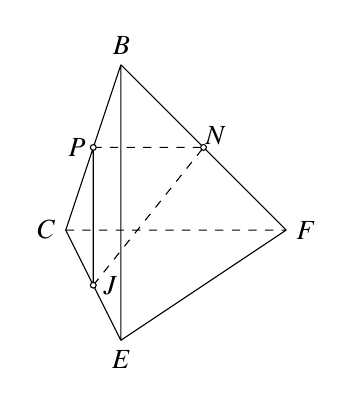
\begin{tikzpicture}[scale=0.7]
				\coordinate (C) at (0,0)   node at (C) [left] {$C$};
				\coordinate (E) at (1,-2) node at (E) [below] {$E$};
				\coordinate (F) at (4,0)   node at (F) [right] {$F$};
				\coordinate (B) at (1,3)   node at (B) [above] {$B$};
				\coordinate (P) at ($(B)!0.5!(C)$);
				\coordinate (J) at ($(C)!0.5!(E)$);
				\coordinate (N) at ($(B)!0.5!(F)$);
				\draw [dashed] (C)--(F) (P)--(N) (J)--(N); 
				\draw (C)--(E) (E)--(F) (B)--(C) (B)--(E) (B)--(F) (P)--(J) ;
				\foreach \i/\g in {P/180, J/0,N/45}{\draw[fill=white](\i) circle (1.5pt) ($(\i)+(\g:3mm)$) node[scale=1]{$\i$};}
			\end{tikzpicture}
			
		\end{center}
		$PN//(JEF)$ là khẳng định đúng. 
}\end{ex}







\newpage 



\end{document}